\documentclass{article}
\usepackage[utf8]{inputenc}
\usepackage{amsmath}
\usepackage{graphicx}
\usepackage[a4paper, margin=1in]{geometry}



\title{Link Scheduling Notes}
\author{mdskrzypczyk }
\date{August 2019}

\begin{document}

\maketitle

\section{Device notes}
\begin{itemize}
    \item Matteo says that any NV device can be brought to the $T_1/T_2$ parameters used in the link layer simulations through careful tuning.
    \begin{itemize}
        \item Might mean it's worth focusing on a homogenous network of nodes that decohere at the same rate. This means that only the initial fidelity matters depending on the distance of the links.
        \item SWAP'd links will then degrade at the same rate as the individual ones between nodes, can apply an exponential fitting to track the loss of fidelity.
    \end{itemize}
    \item Also said that the parameters may fluctuate between 30\% and 100\% of those used in the simulations, so can also investigate heterogenous networks.
    \item Consider storing the links with better fidelity first in the carbon due to the great storage time.  This will \emph{probably} maximize the resulting swapped fidelity.
\end{itemize}

\subsection{Decoherence for single/double electron/carbon storage}
\begin{figure}[!htb]
    \centering
    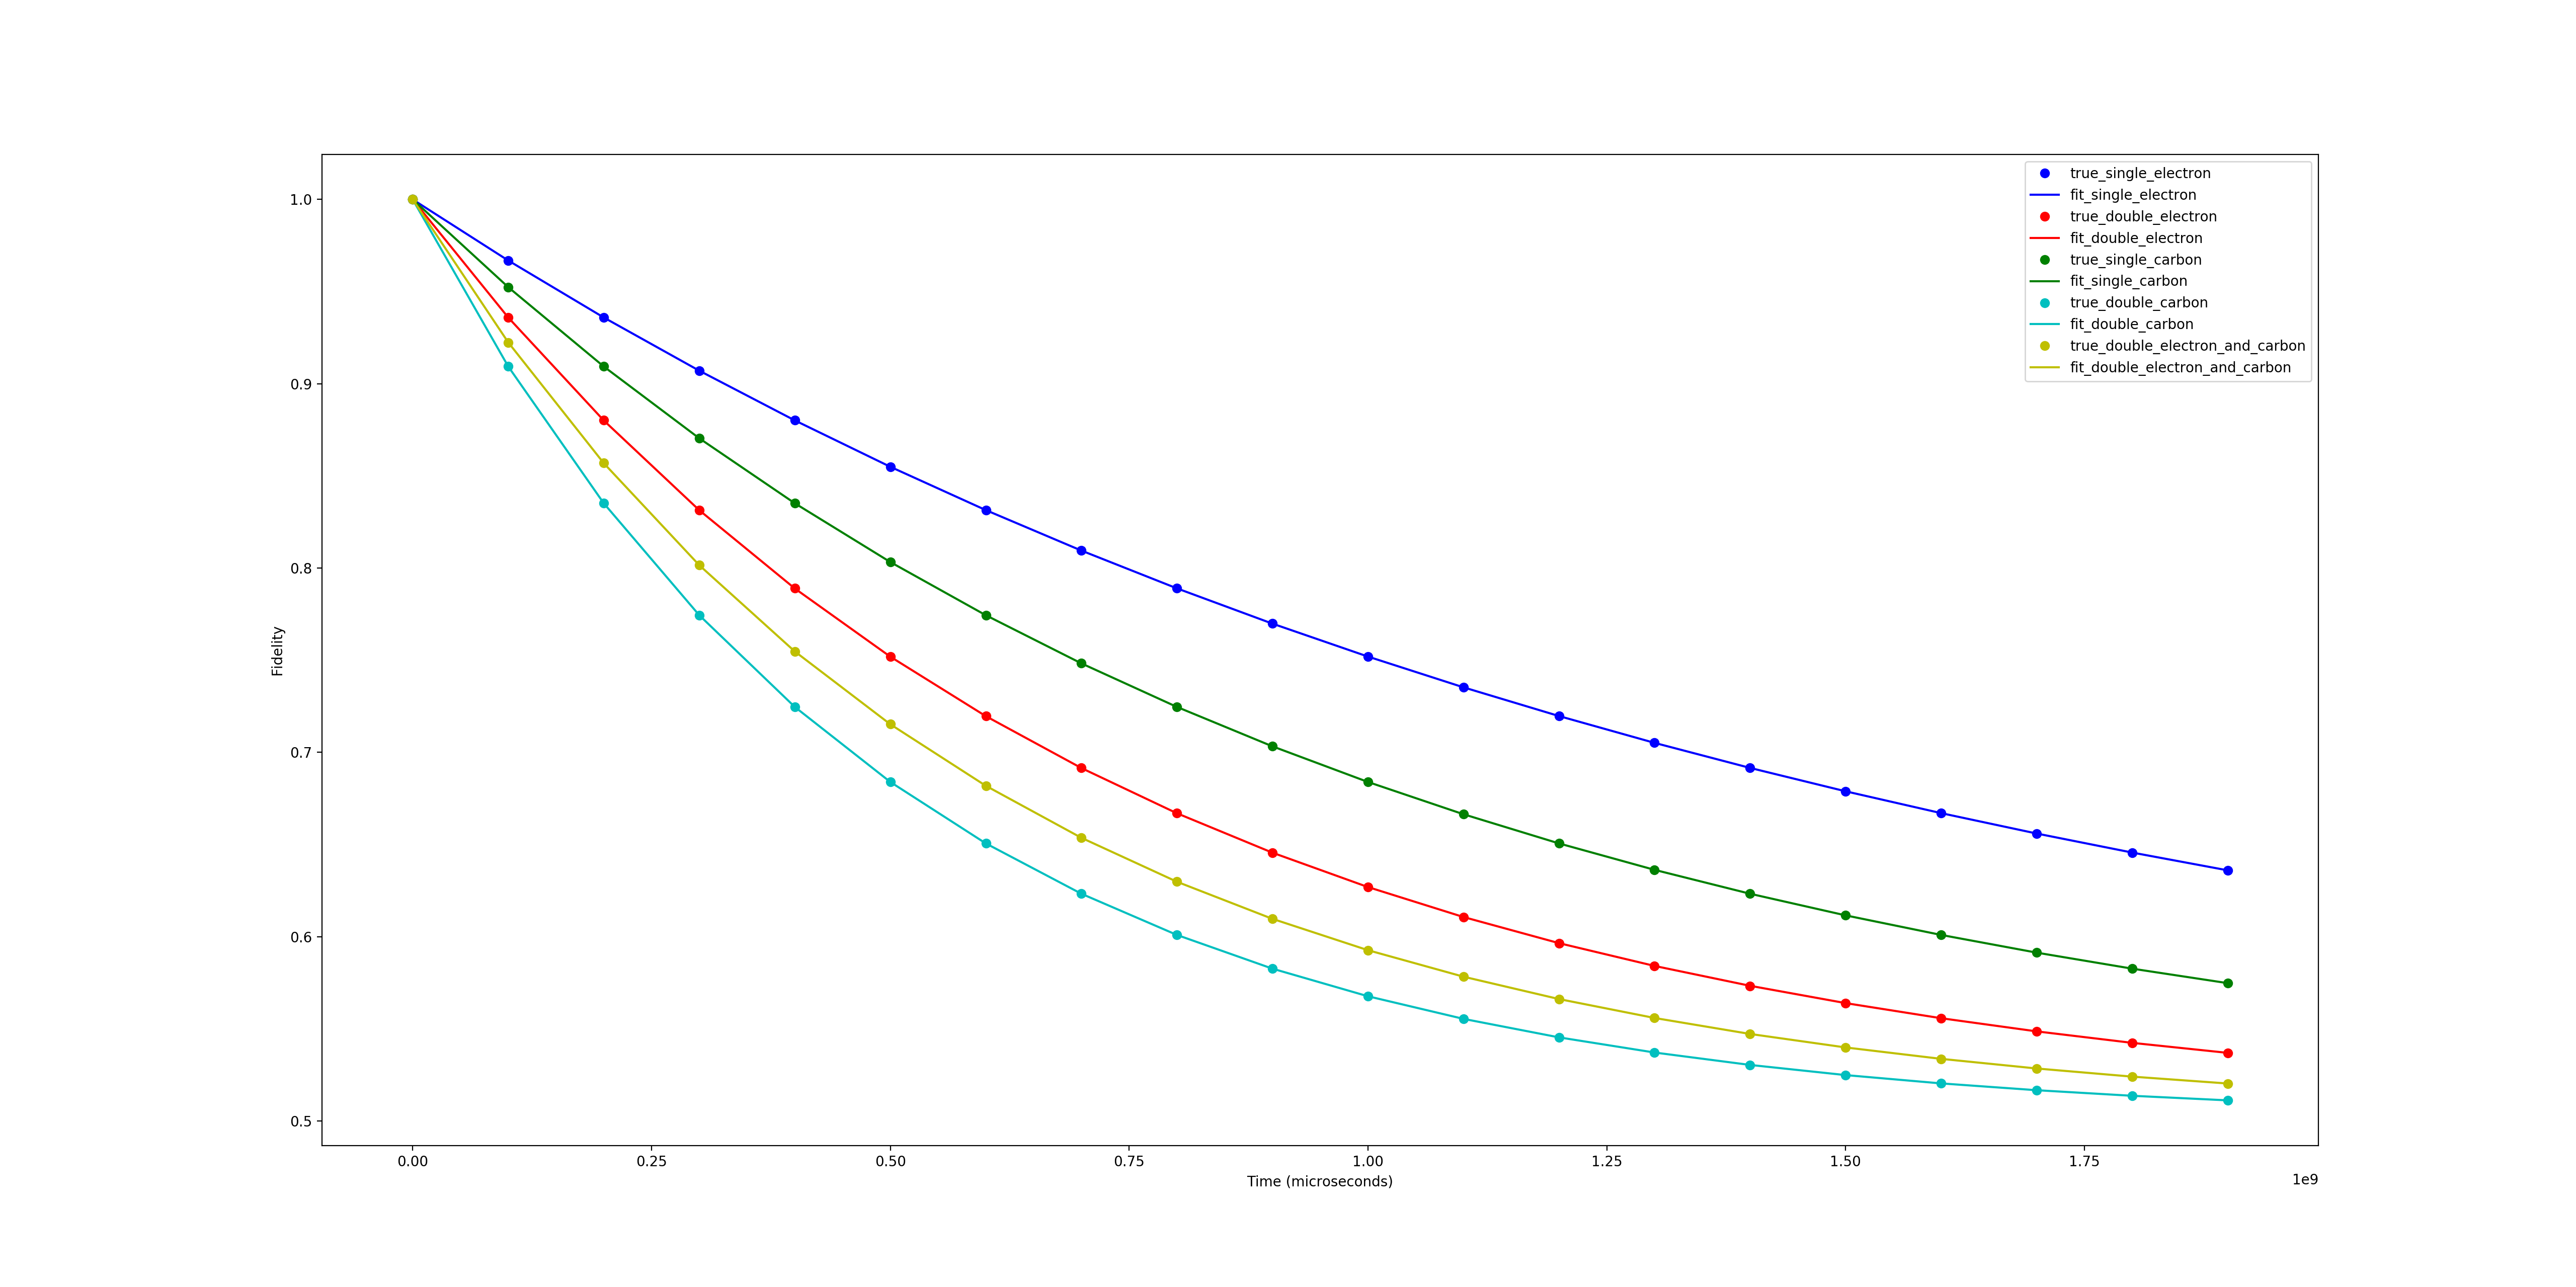
\includegraphics[width=\textwidth]{figures/decoherence.png}
    \caption{Plot of decoherence on an entangled pair of qubits for cases where a single qubit is in the electron/carbon and the other is stored perfectly, both are in the electron, both are in the carbon, and one in electron while other in carbon. All bell pairs initiated at $F=1$ with move to storage performed immediately after generating.}
    \label{fig:decoherence}
\end{figure}

This plot was generated using the following values for $T_1/T_2$ times sourced from the experimental realizations discussed in \emph{A Link Layer Protocol for Quantum Networks}.

\begin{table}[!htb]
\centering
\begin{tabular}{|l|l|l|l|l|}
\hline
              & Electron $T_1$ & Electron $T_2$ & Carbon $T_1$ & Carbon $T_2$ \\
\hline
Duration/Time & 1h            & 1.46s       & 10h ($\inf$) & 1s          \\
\hline
\end{tabular}
\end{table}

From the collected data it also appears that if we fit the curves with $f=ae^{-bt}+c$ for storage in electron/electron, carbon/carbon, and electron/carbon, we can compute the single electron/carbon decoherence using the same $a,c$ but computing $b_{single}=
\frac{1}{2}b_{double}$ and obtaining $b_{double}$ for electron/carbon by simply summing $b_{single}$ for both the electron and carbon decoherence.

Additional plots of decoherence consider inserting a delay before the SWAP occurs from the electron to the carbon.
\begin{figure}[!htb]
    \centering
    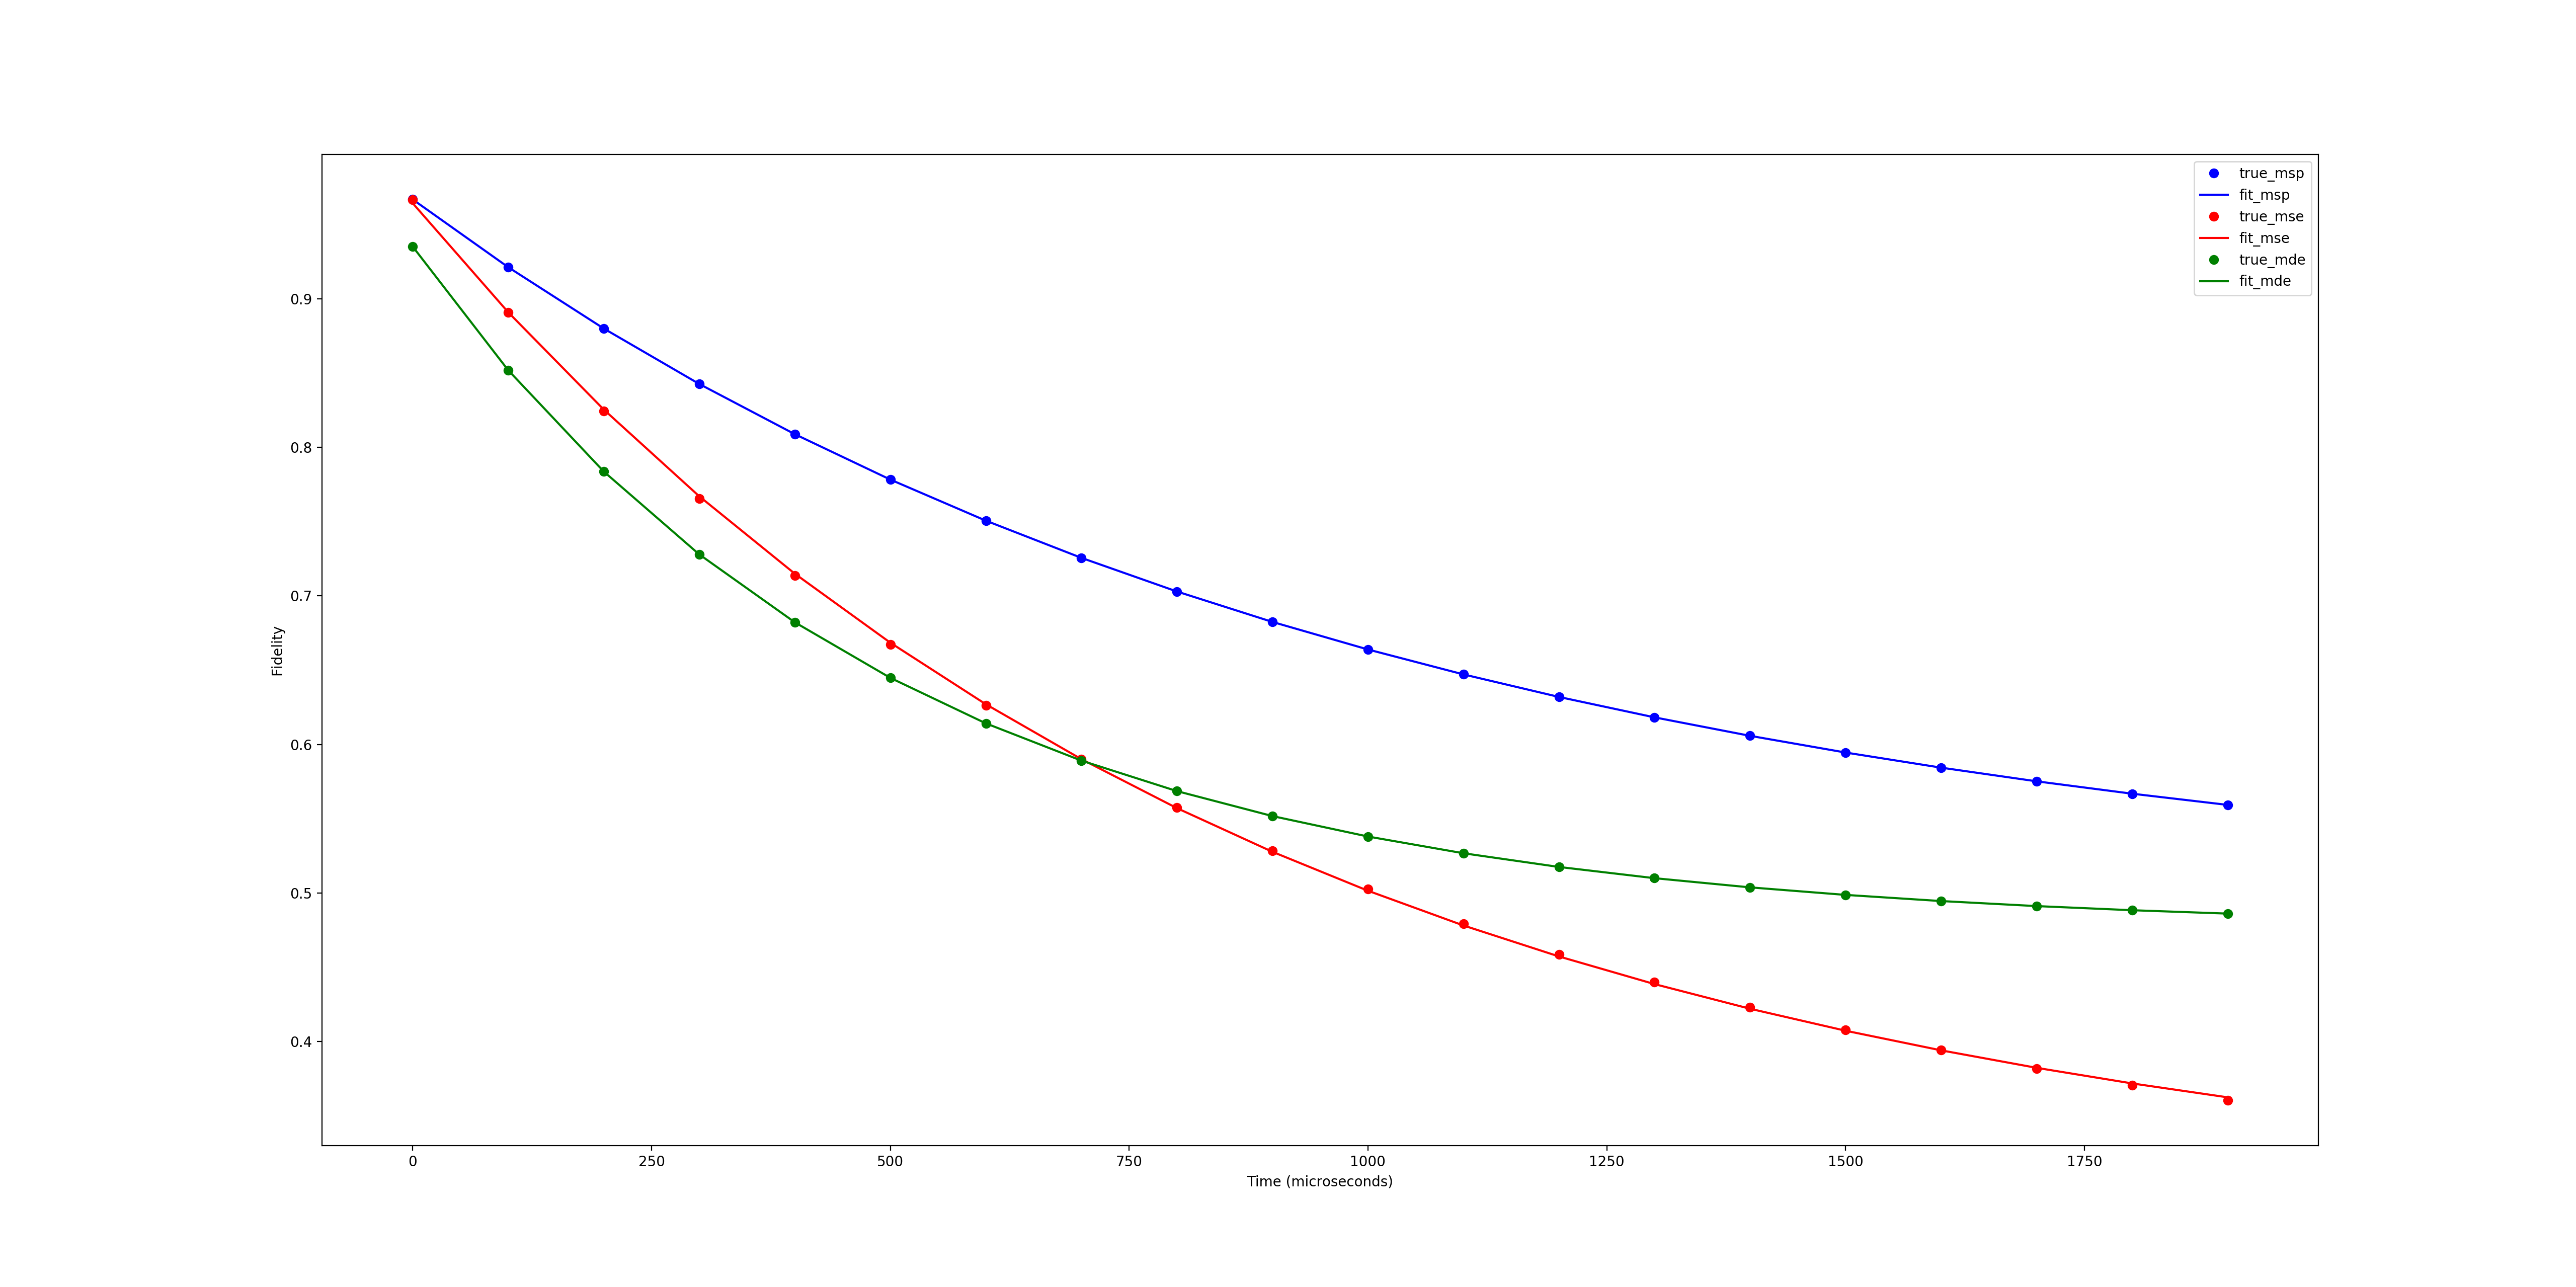
\includegraphics[width=\textwidth]{figures/decoherence_move_delay_0ms.png}
    \caption{Plot of decoherences with move delay of $100ms$.}
    \label{fig:decoherence_0_delay}
\end{figure}

\begin{figure}[!htb]
    \centering
    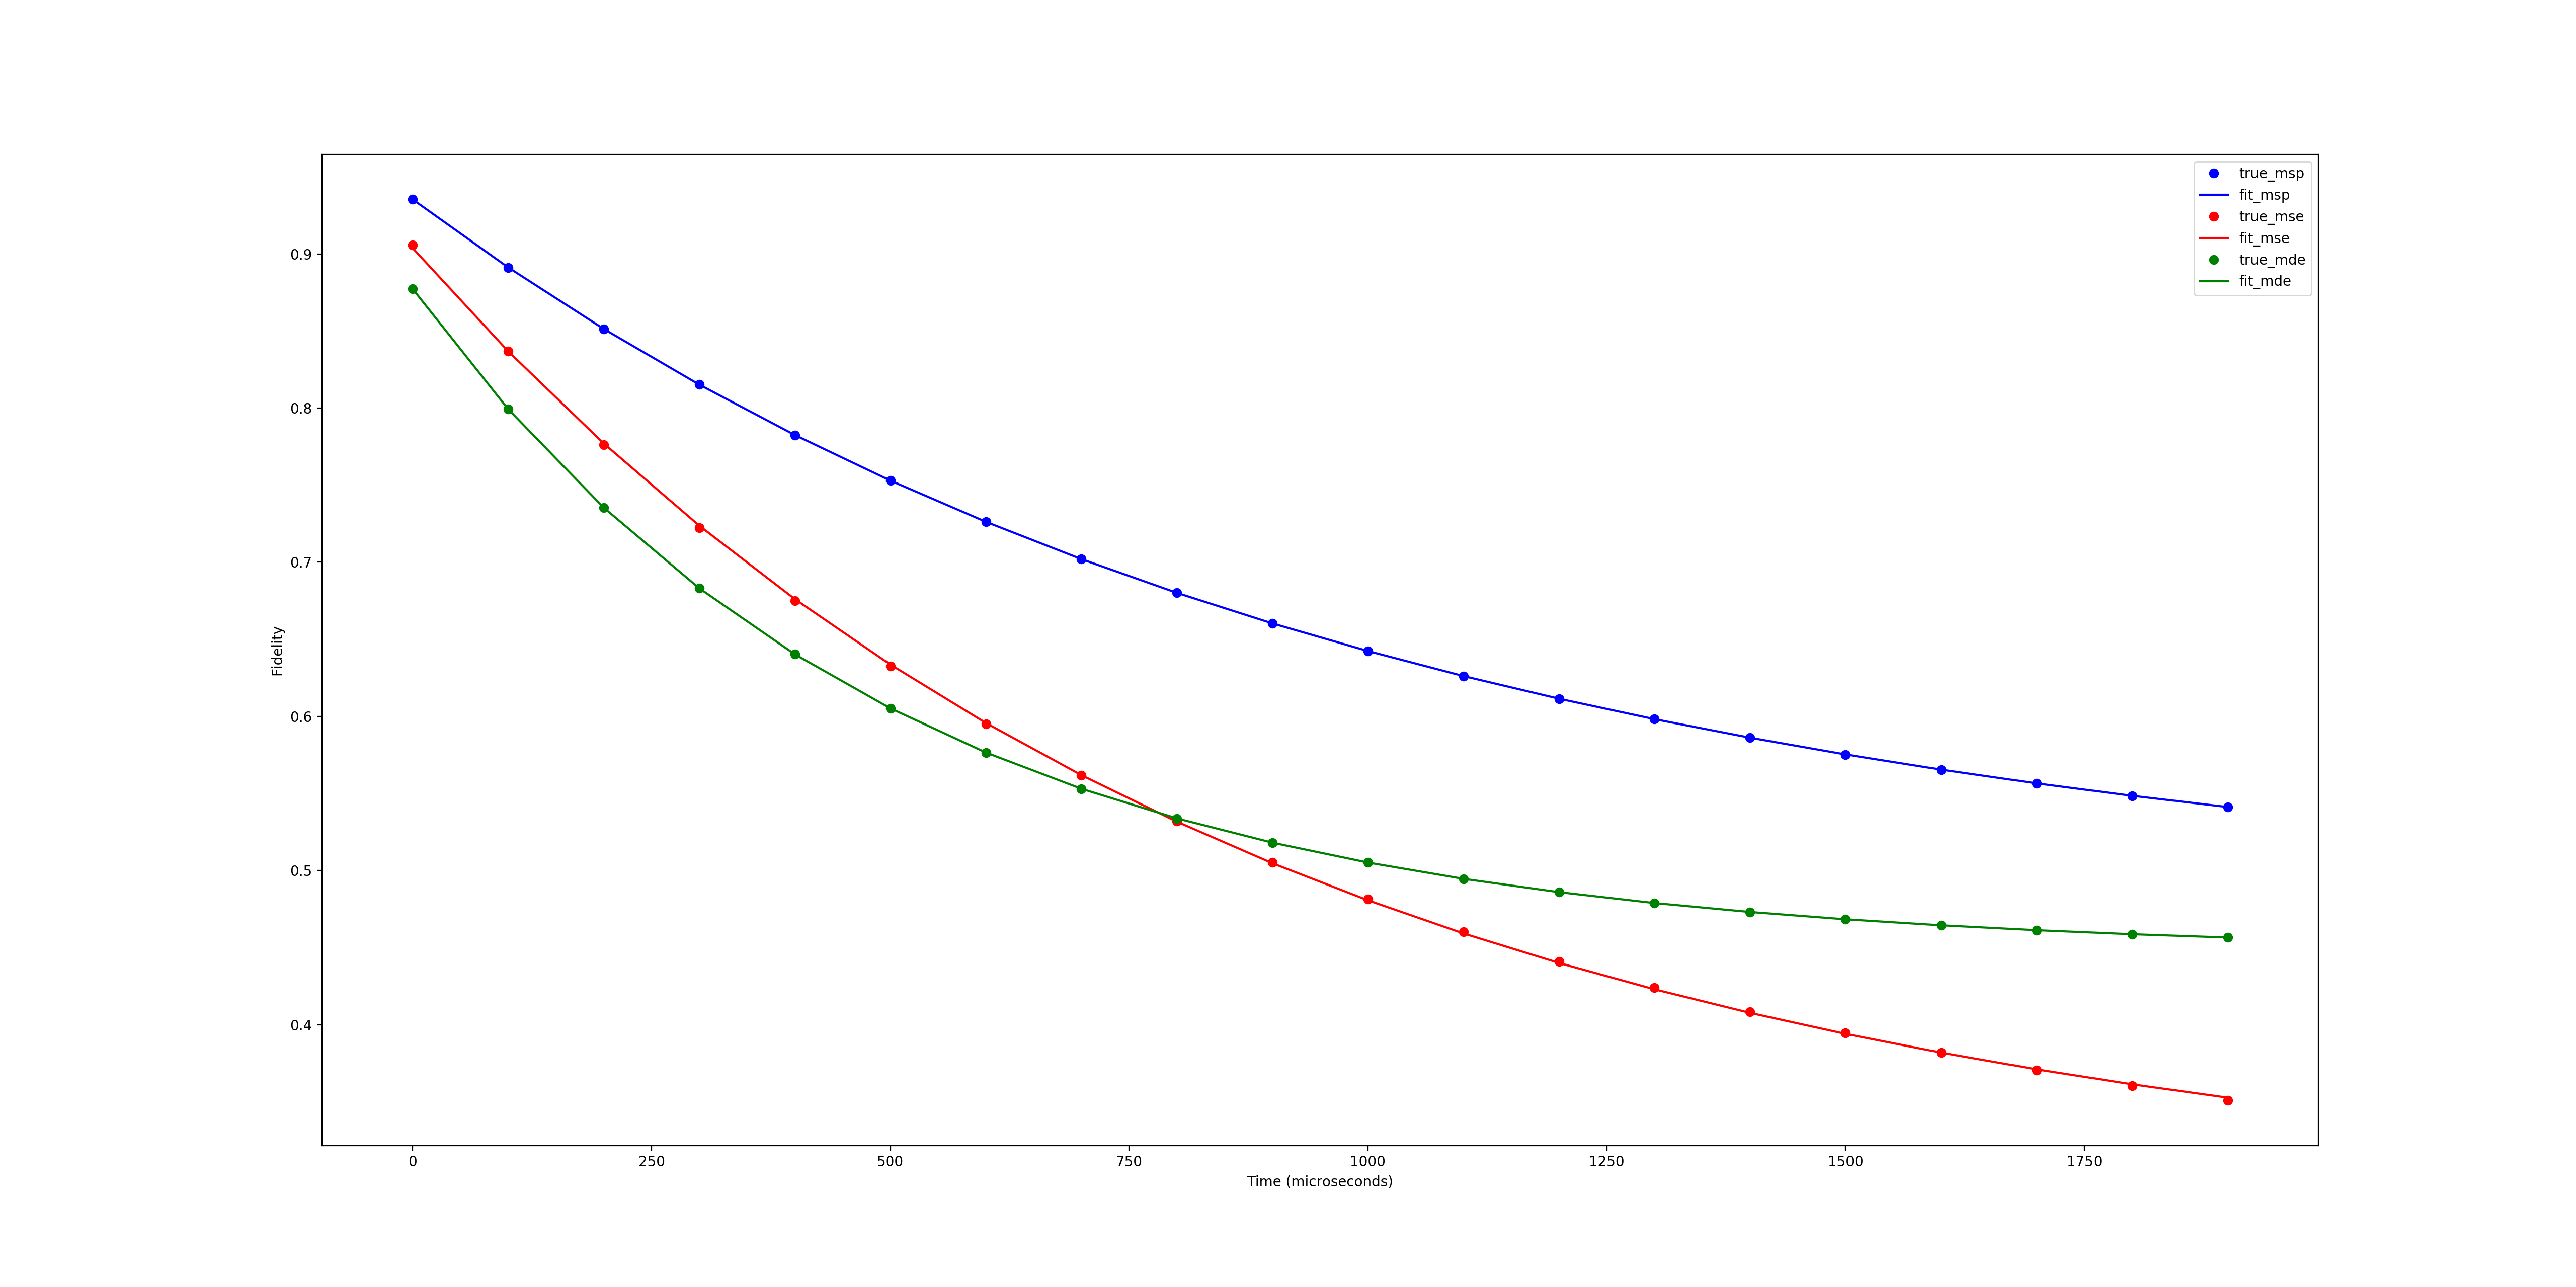
\includegraphics[width=\textwidth]{figures/decoherence_move_delay_100ms.png}
    \caption{Plot of decoherences with SWAP delay of $100ms$.}
    \label{fig:decoherence_100_delay}
\end{figure}

\begin{figure}[!htb]
    \centering
    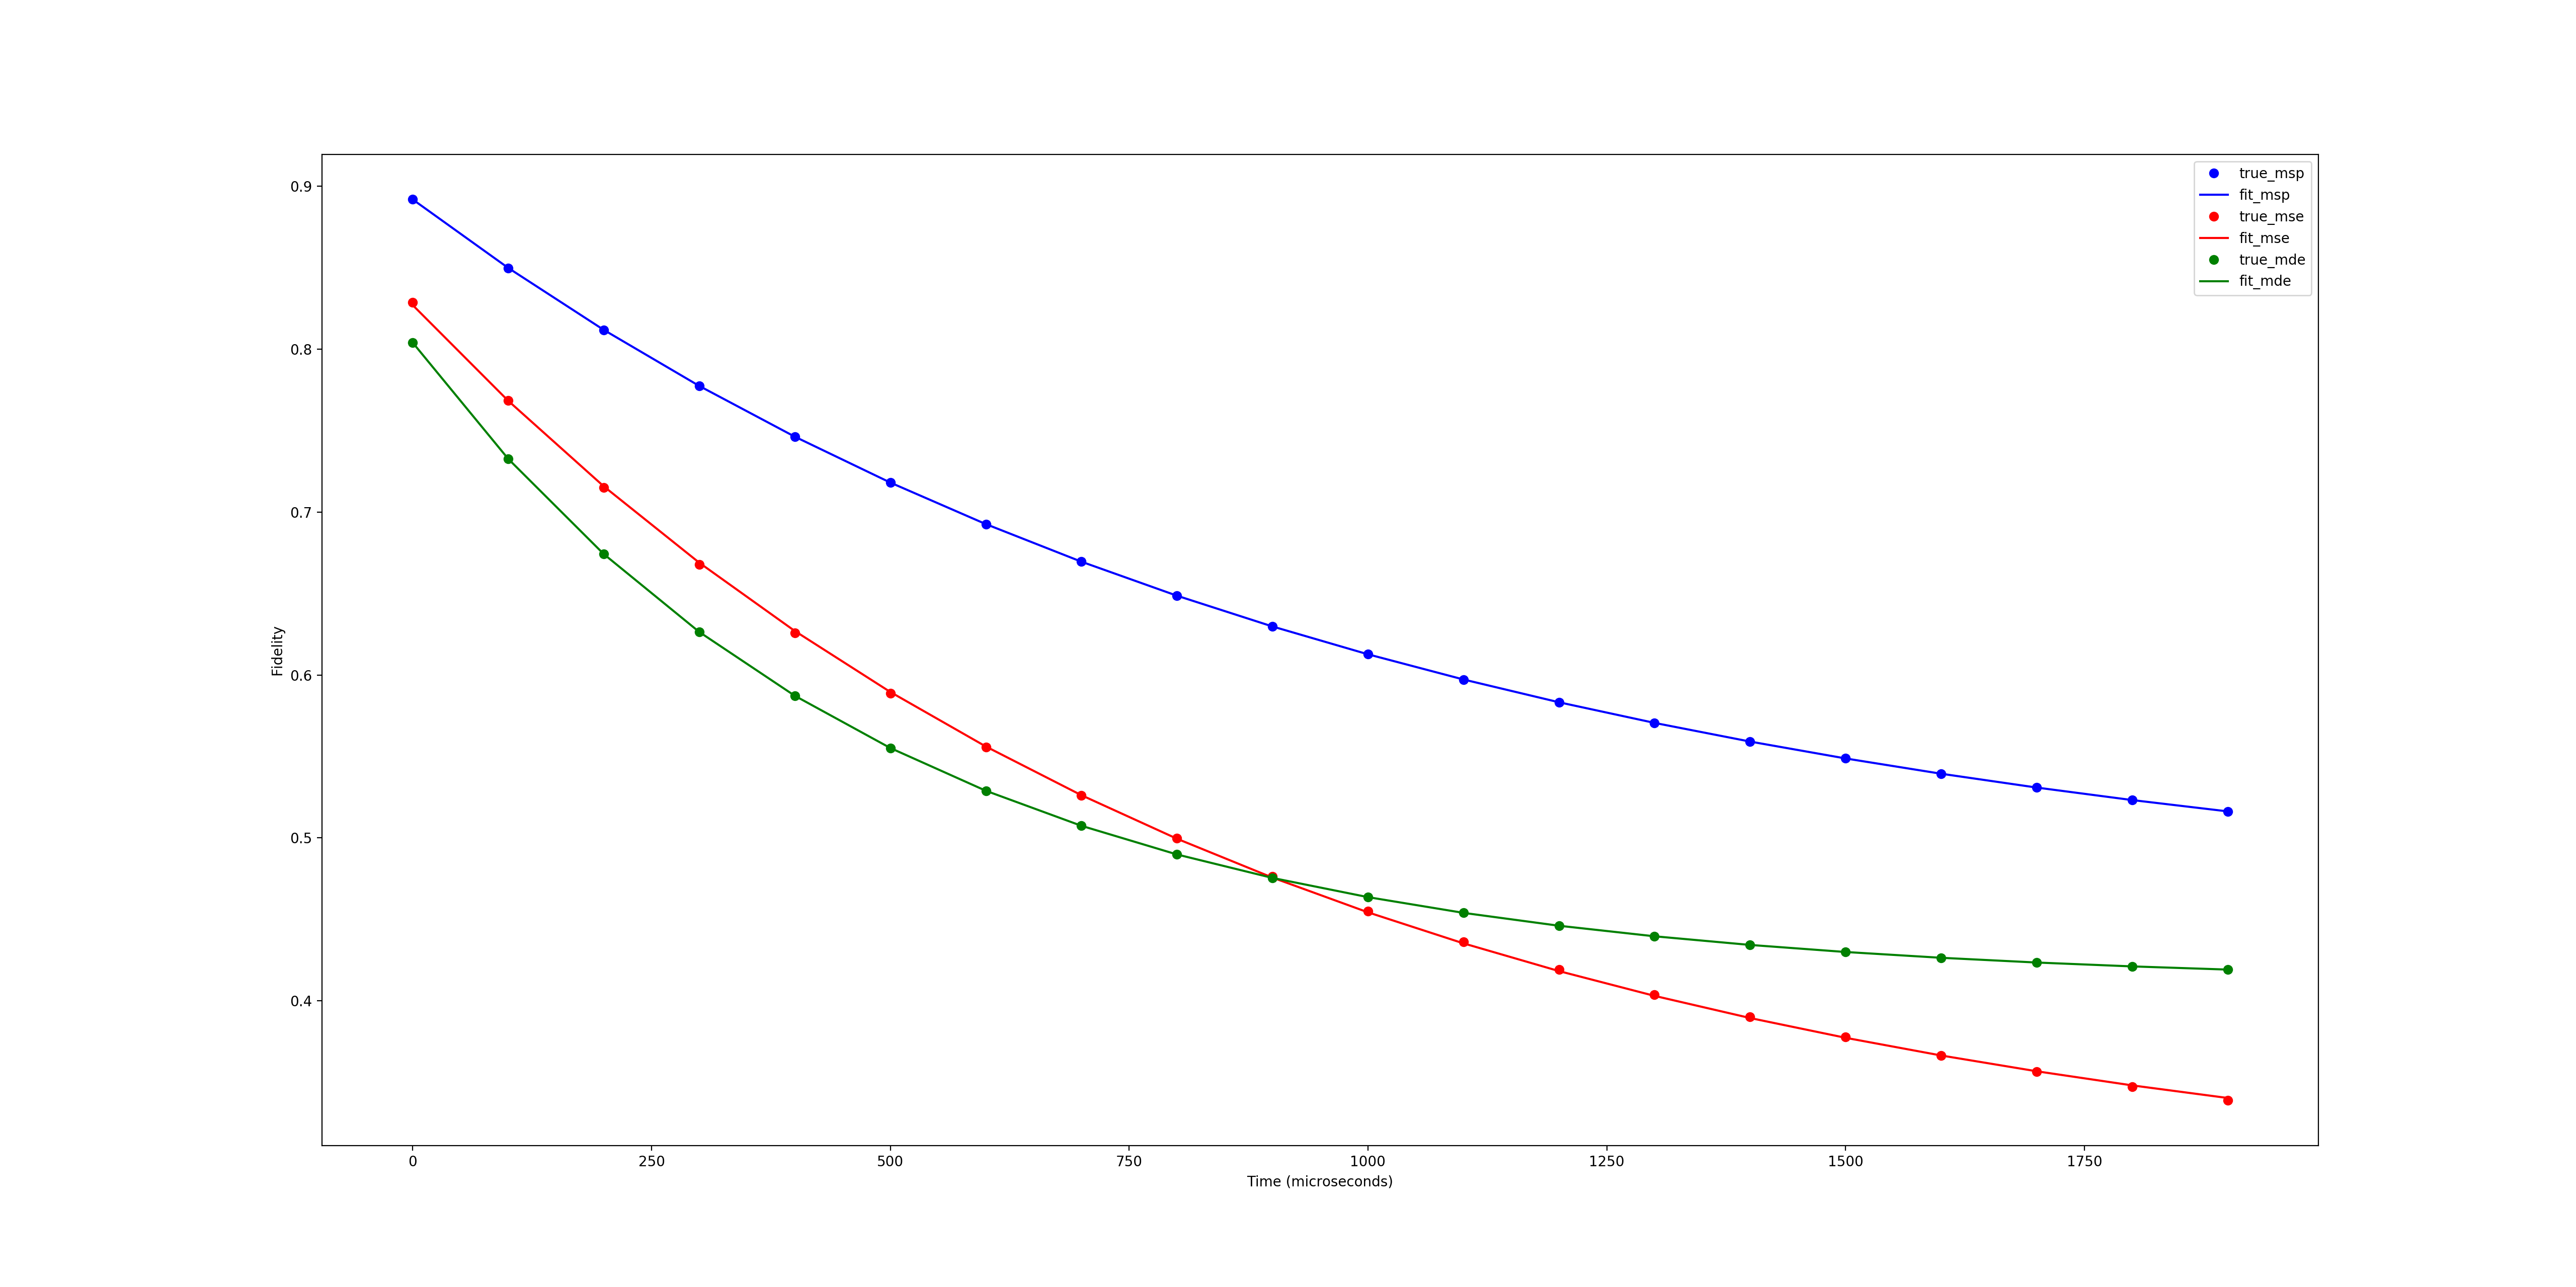
\includegraphics[width=\textwidth]{figures/decoherence_move_delay_250ms.png}
    \caption{Plot of decoherences with move delay of $250ms$.}
    \label{fig:decoherence_250_delay}
\end{figure}

\begin{figure}[!htb]
    \centering
    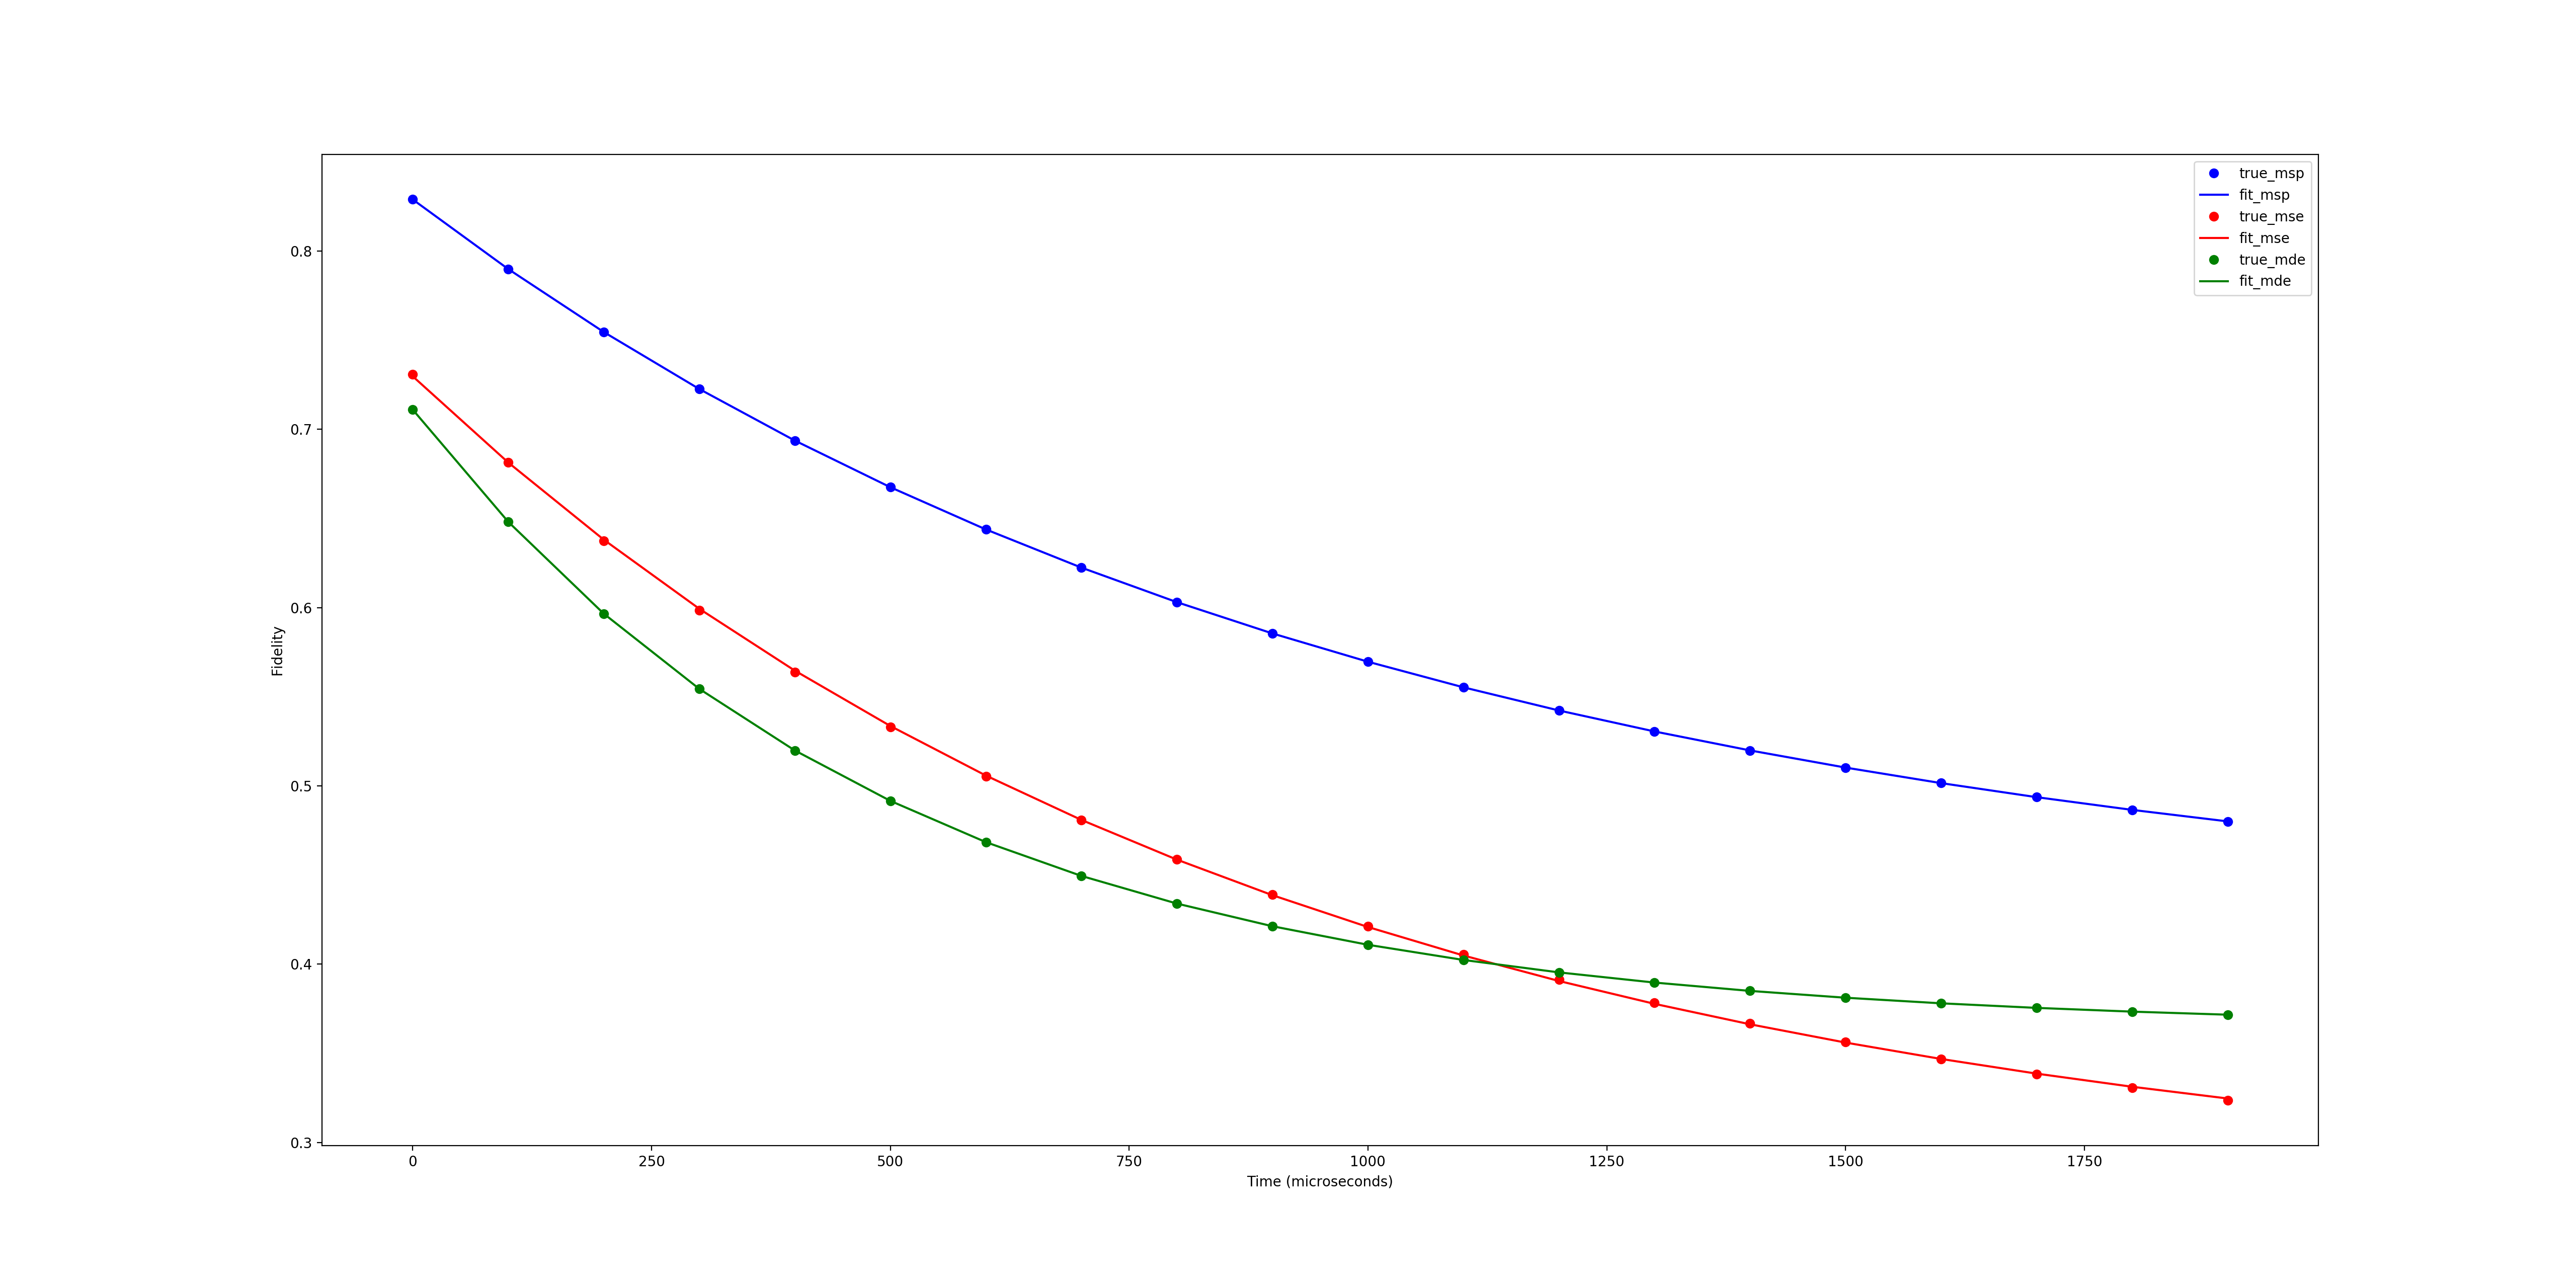
\includegraphics[width=\textwidth]{figures/decoherence_move_delay_500ms.png}
    \caption{Plot of decoherences with move delay of $500ms$.}
    \label{fig:decoherence_500_delay}
\end{figure}

\begin{figure}[!htb]
    \centering
    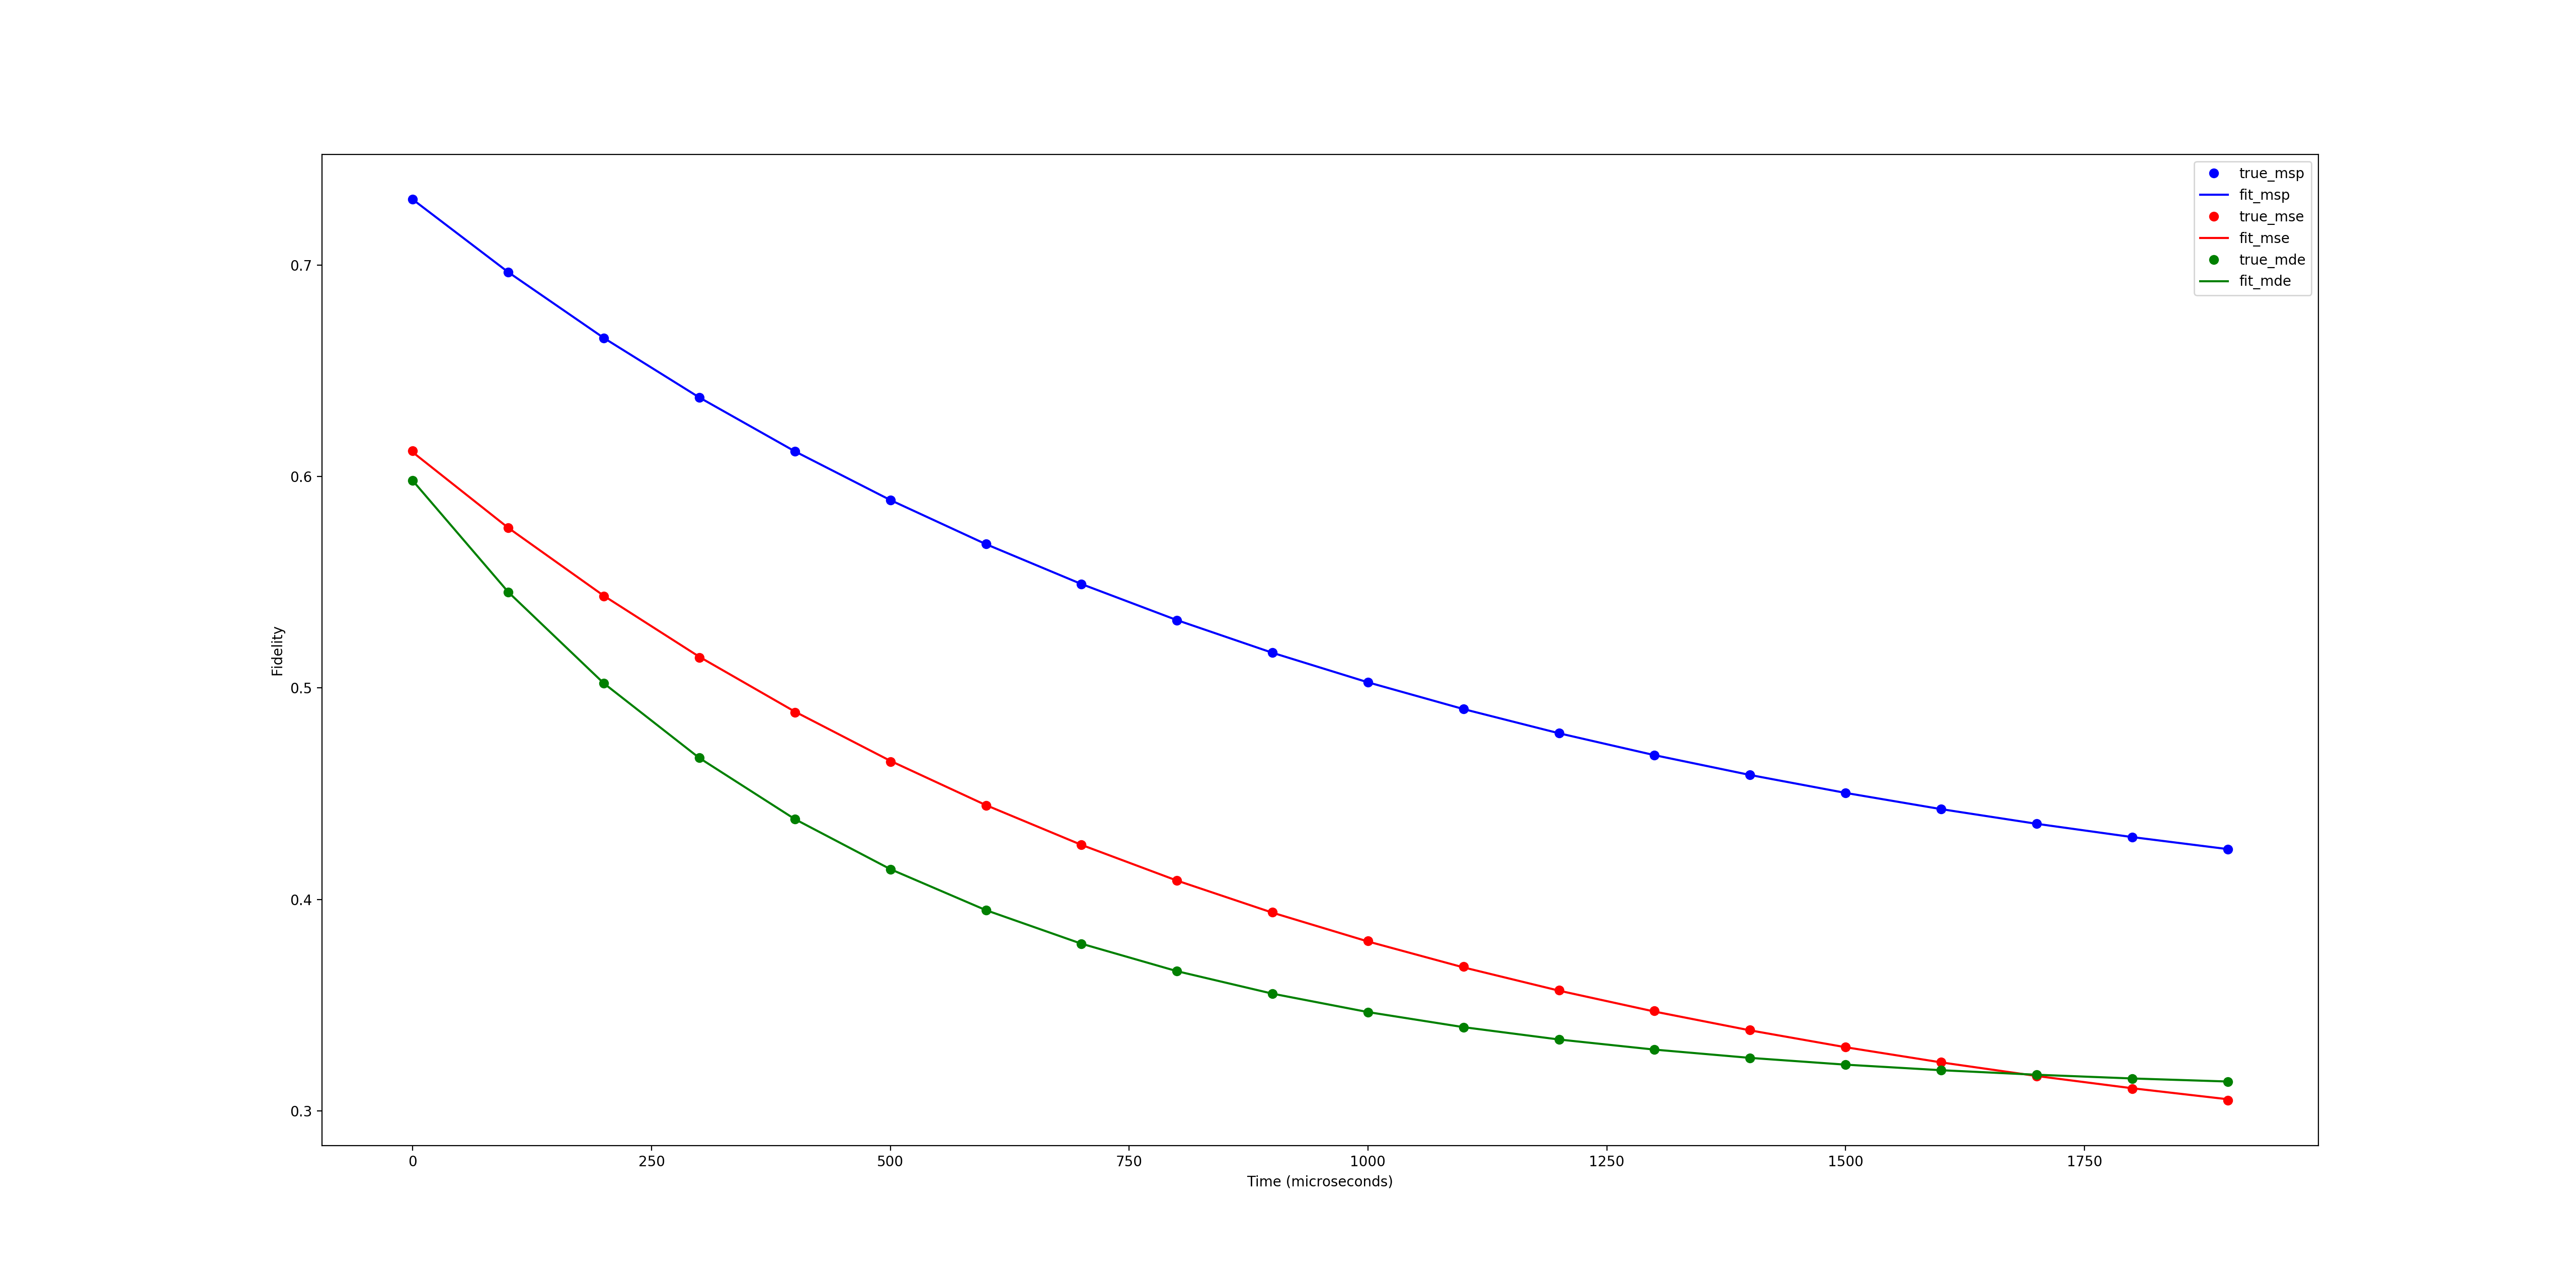
\includegraphics[width=\textwidth]{figures/decoherence_move_delay_1000ms.png}
    \caption{Plot of decoherences with move delay of $1000ms$.}
    \label{fig:decoherence_1000_delay}
\end{figure}

\begin{figure}[!htb]
    \centering
    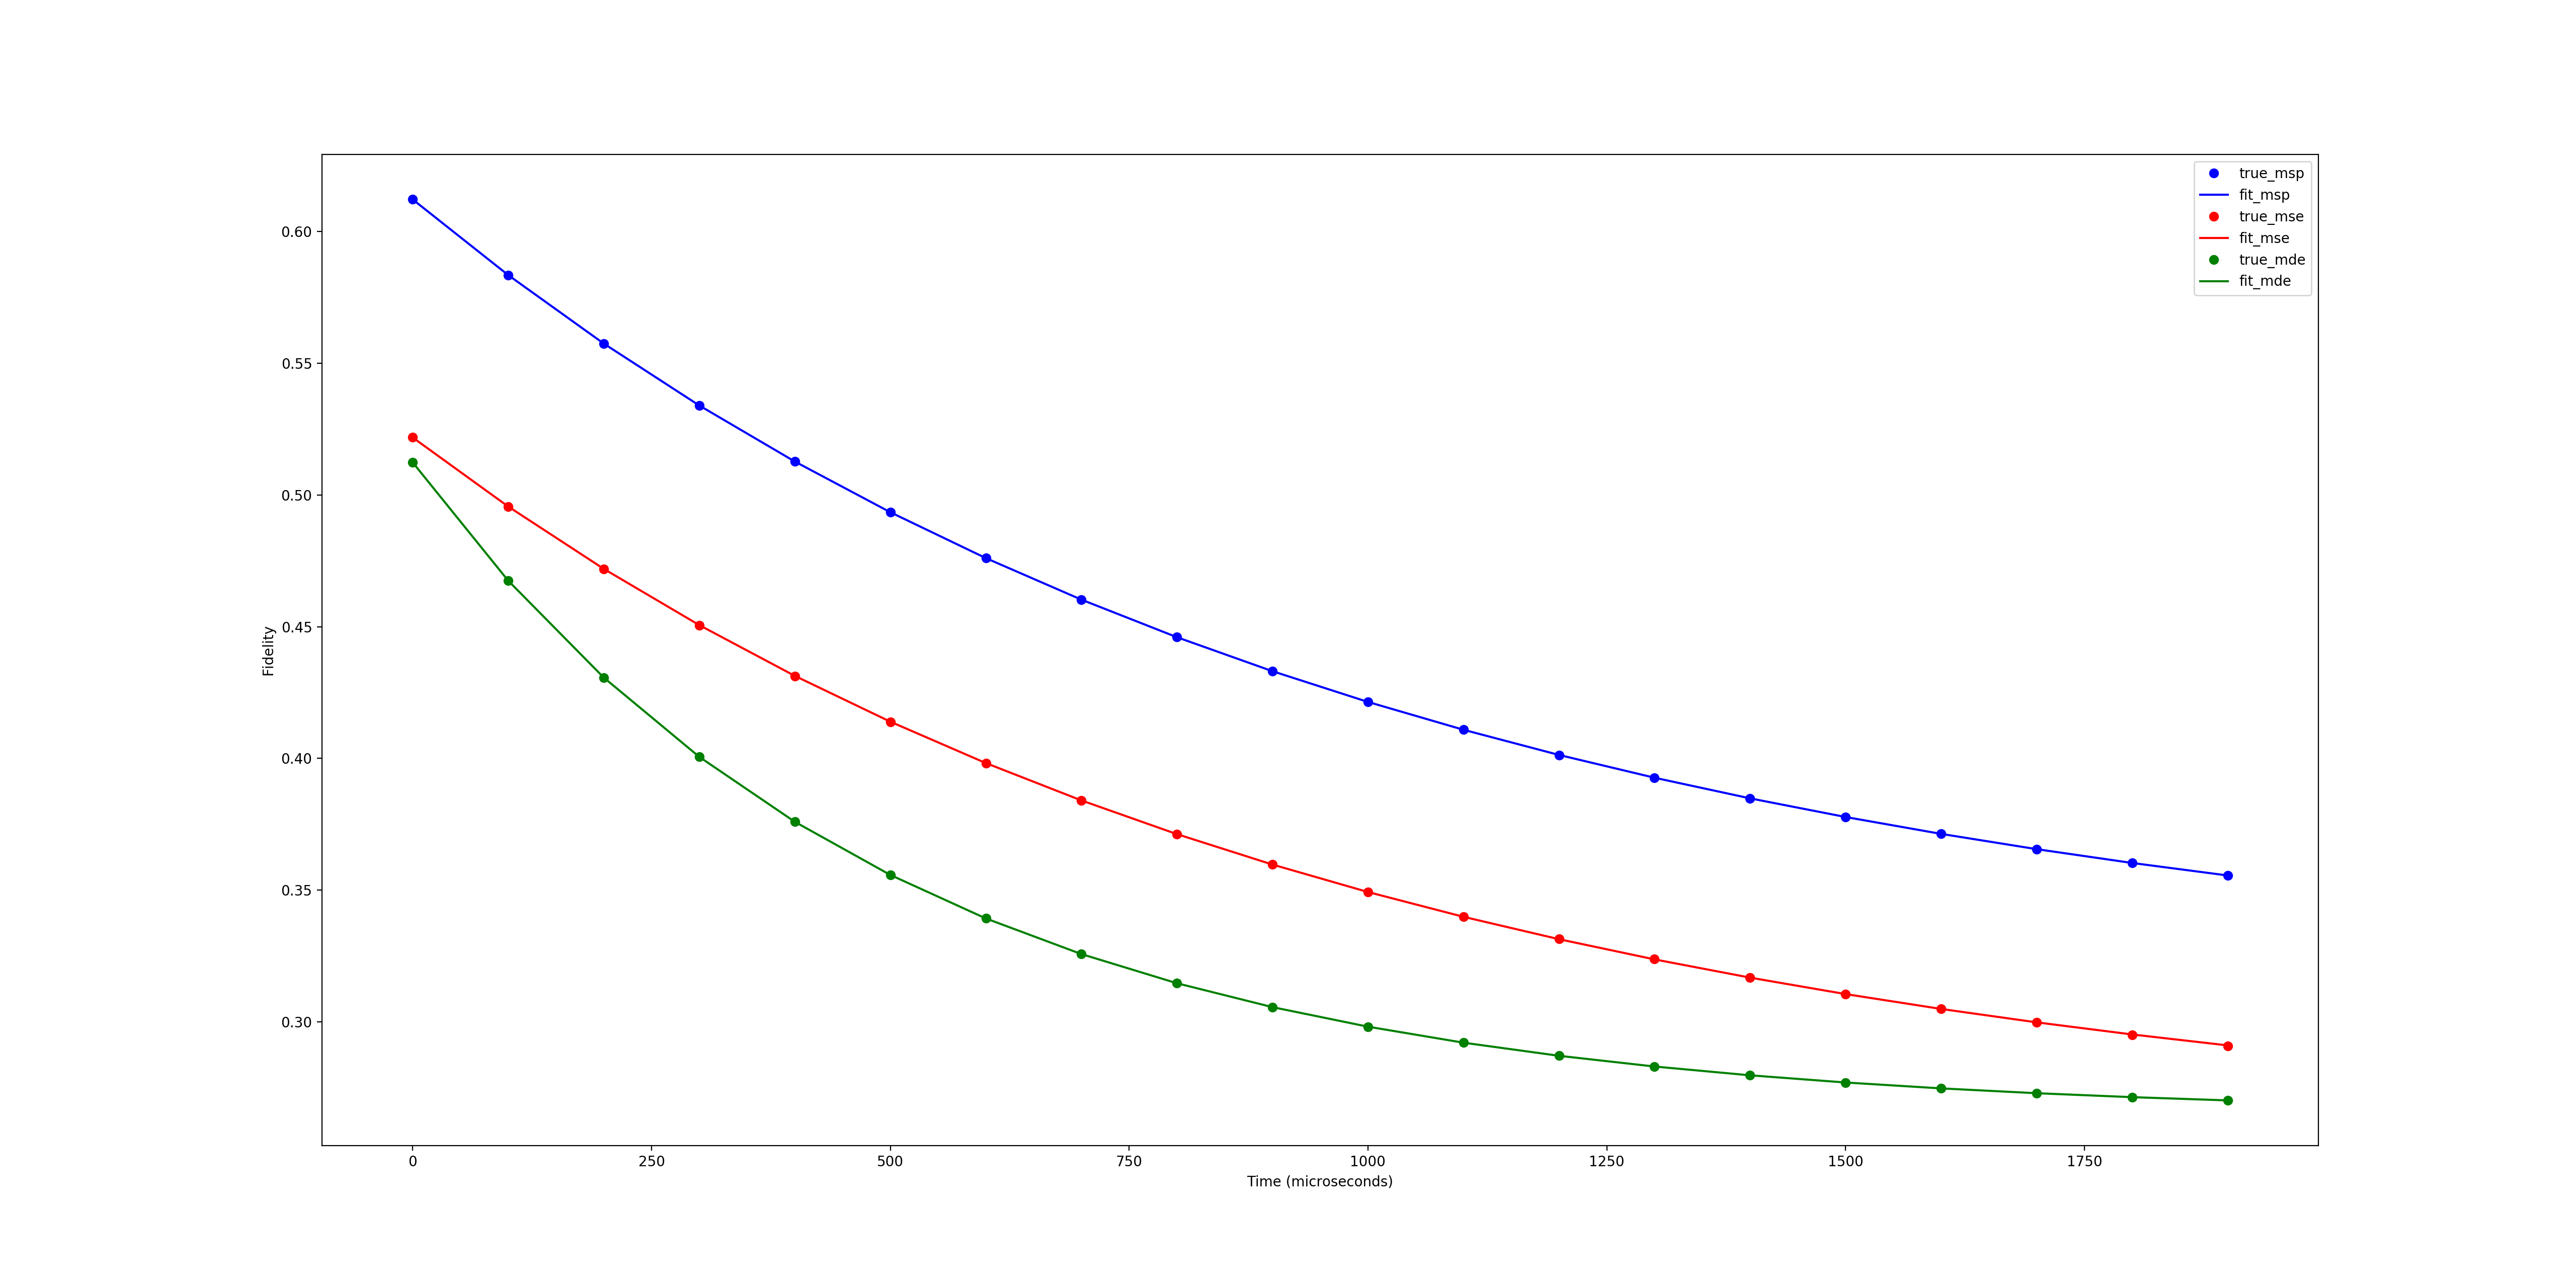
\includegraphics[width=\textwidth]{figures/decoherence_move_delay_2000ms.png}
    \caption{Plot of decoherences with move delay of $2000ms$.}
    \label{fig:decoherence_2000_delay}
\end{figure}

\begin{figure}[!htb]
    \centering
    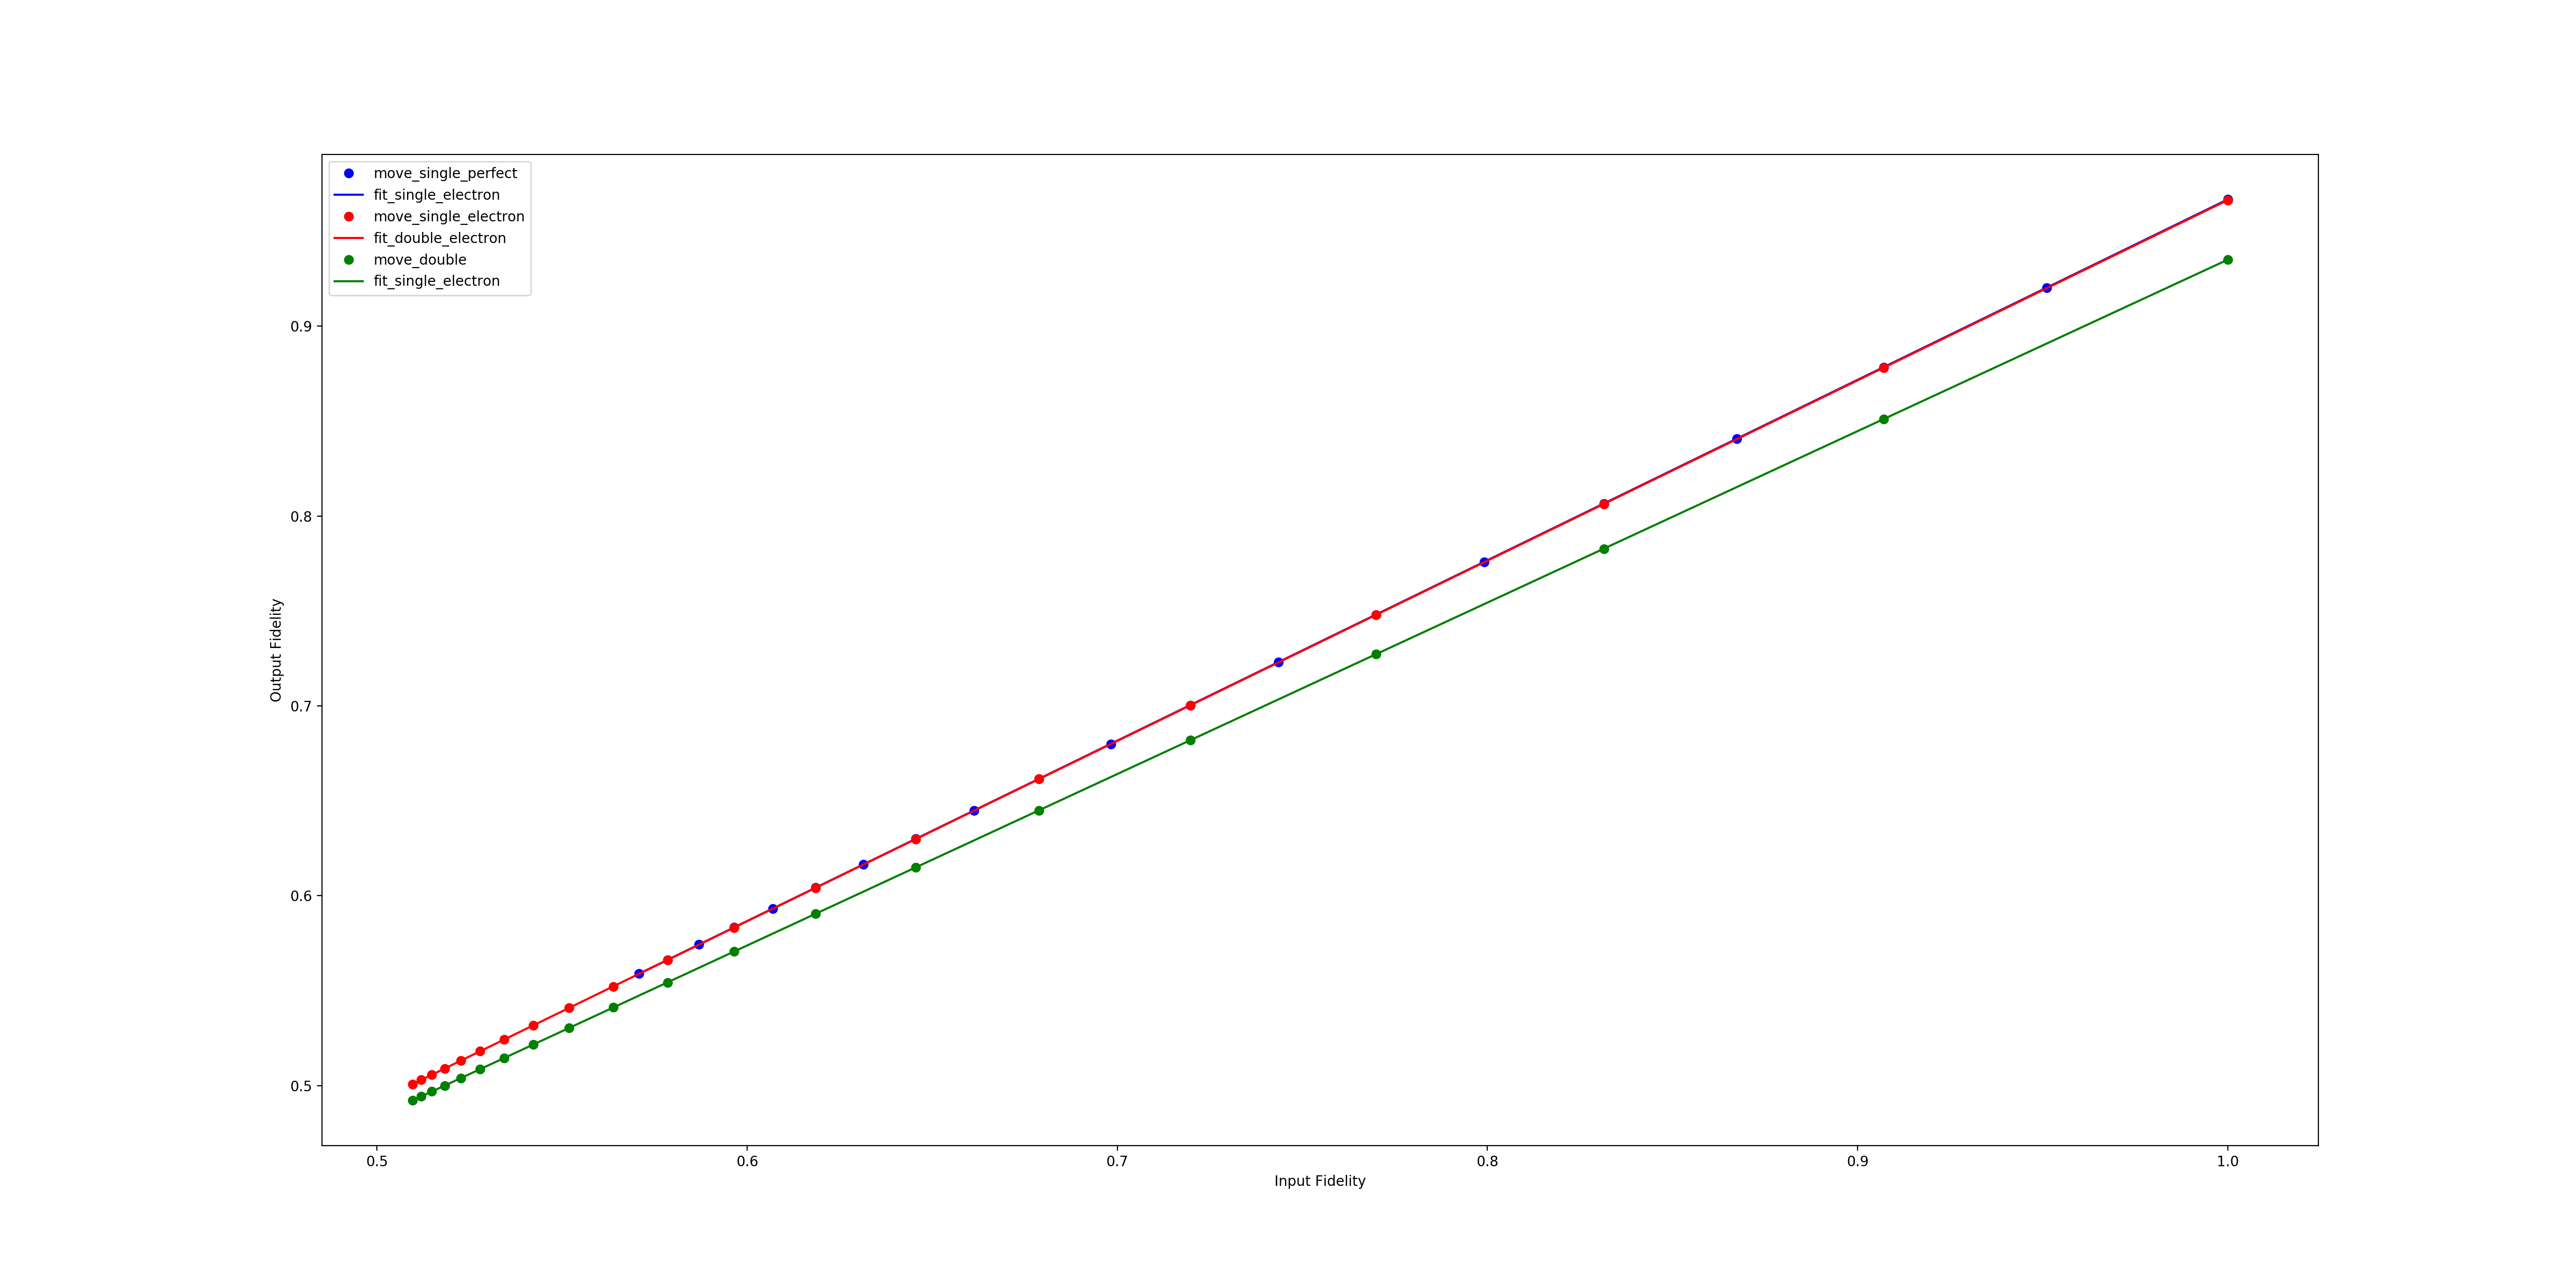
\includegraphics[width=\textwidth]{figures/move_decoherence.png}
    \caption{Plot of initial fidelity/post-move fidelity.}
    \label{fig:decoherence_move}
\end{figure}

Note that the fidelities for moving entanglement into the carbons on both devices actually yields a higher fidelity.  This is because while one move is happening the electron is decohering at the other node.  Should verify that noise during the gate operation can be removed which is how this data was generated.

\section{Cost functions}
Objective functions to optimize with choice of link scheduling.

\subsection{Maximized Final Fidelity}
While it may be overkill, in practice this may reduce the number of requests into the network if the fidelity of the produced entanglement is good enough to not try and request it again (while it is more expensive).

Should take into consideration how fidelity evolves across the entire link due to changes in decoherence rate from SWAP-ing (may not be a problem if we assume a homegeneous device network).

\subsection{Minimized Weighted Idle Time}

    $$\text{min } d = \sum_{i=1}^{n-1} w_{i+1}|e_i - e_{i+1}| + max_i(e_i)(w_1 + w_{n+1}) - w_1e_1 - w_{n+1}e_n$$

Where:
\begin{itemize}
    \item $n$ is the number of edges in the chain
    \item $e_i$ is the time at which link $i$ is expected to be generated
    \item $w_i$ is a decoherence weight associated with node $i$
    \item $\sum$ term represents the weighted decoherence introduced by the nodes internal to the chain (2:n)
    \item $max_i(e_i)$ is the completion time of the last link
    \item Final terms represent the decoherence introduced on the qubits held by the end nodes as they must wait until the full link has been established to begin using
\end{itemize}

Observations:
\begin{itemize}
    \item Preferable to have end links generated last as generating them earlier accumulates more decoherence (dependent on weights)
\end{itemize}

\subsection{Minimized Total Fidelity Loss}

$$\text{min } F_{loss} = \sum_{i=1}^{n} F_{0,i}e^{-w_it_i}$$

Where:
\begin{itemize}
    \item $F_{loss}$ is the total lost fidelity
    \item $F_{0,i}$ is the initial fidelity of a generated link
    \item $w_i$ is the rate of decoherence of a link
    \item $t_i$ is the amount of time the link decoheres for
\end{itemize}

Problems:
\begin{itemize}
    \item Metric does not consider how the links decohere after they have been SWAPPED, $w_i$ is a property of the
    originally generated link, not the nodes holding the qubits
\end{itemize}

\section{Greedy Heuristics}
\begin{itemize}
    \item Place links that take less time to generate ahead of current link and links that take less time behind the current link.
    \begin{itemize}
        \item Can this actually put us in a position where decoherence puts fidelity of a link too low to be useful?
    \end{itemize}
    \item Place links that have a higher fidelity by the time both links should be done earlier in the schedule
\end{itemize}

\section{Coordination}
\subsection{Timeslot Scheduling}
Share schedules of nodes along path and insert slots for when time should be spent generating a link.

\subsubsection{Why Timeslot Scheduling?}
\begin{itemize}
    \item We want a coordination mechanism that can take into account a node's availability to establish entanglement in the network.
    \item This may include applications that are running at the node which cannot be interrupted or other links the node is helping establish.
    \item We also want to reduce additional communication for coordinating link building, ie. avoid communication between nodes of the form "I am done with link X are you available to start link Y?" as this might go on indefinitely.
    \item Timeslot scheduling allows us a simple mechanism to stop generating a link.  If we have not generated a shorter segment by the end of the slot, we give up and can instruct other nodes to give up as well.
    \item Timeslot scheduling can be done in a centralized manner where an external central authority knows all the schedules of the nodes or requests them or it can be done in a distributed manner where the nodes along the path share their schedules with one another.
\end{itemize}

\subsubsection{Execution Techniques}
\begin{itemize}
    \item Get individual machine schedules.
    \begin{itemize}
        \item Schedule cannot be represented infinitely into the future (messages are finite in size, base size on the max time of generation request?
        \item Need an efficient representation that permits taking intersections for creating link schedules
        \item Prune slots that are occupied or too short for generating a given link.  "Too short" can have a few meanings, below average or below some fraction of average time to generate. (Check probability distribution, geometric?)
        \item Represent schedule for each communication qubit on the link
    \end{itemize}
    \item Take an intersection to form availability schedules for each link.
    \begin{itemize}
        \item How can we take into account several communication qubits for this part?
        \item Reserving a slot in a link schedule affects the adjacent link schedule availability.
    \end{itemize}
    \item Determine the order of the links and which slots should be used.
    \begin{itemize}
        \item Prune to isolate valid pairs of adjacent slots that allow SWAP-ing to achieve reasonable fidelity.
        \begin{itemize}
            \item "Window" adjacent schedules to find pairs of slots.  Window size should tolerate occupied slots between available slots.  May be based on achievable fidelity and how low we can accept the fidelity to become before the second link generates.
            \begin{itemize}
                \item Use $F_{SWAP}=F_1 F_2 + \frac{(1-F_1)(1-F_2)}{3}$, if windowing links in the past, set $F_1$ to the fidelity produced of the previous link, set $F_2=ae^{-w(t_0+t)} + c$ with $t_0$ corresponding to the initial link fidelity, compute maximum $t$ such that $F_{SWAP} \geq F_T$ where $F_T$ is some lower threshold on the needed fidelity.  Only consider links in the past that complete within $t$ time before previous link is \emph{finished} generating.
                \item If windowing in the future, set $F_2$ to the initial fidelity of the next link and compute $F_1=ae^{-w(t_0+t)}+c$ similarly. Similar to above but treat the previous link as the one in the past and see how far into the future you can generate a link.
            \end{itemize}
            \item Can we order these slot pairs by a greedy heuristic?
            \item Can also order based on how much faster/slower a link would degrade the sooner we can push a SWAP through to a device that decoheres less.
        \end{itemize}
        \item There may be several "starting" points within a link availability schedule, how to pick which one?
        \begin{itemize}
            \item Consider the timespan of generating all the links?
            \item Construct a naive order assuming full availability and then slot?
            \item Construct the order based on the available slots?  Start with the earliest slot?  Start with the worst link?
            \item Brute force is $O(l2^n)$ if an end node's schedule has $l$ starts and we use the closest two slots (before/after) for $n$ nodes
            \item Greedy has $O(nl)$ if an end node has $l$ different starts and we always select the next one simply
        \end{itemize}
        \item In order to calculate fidelities, can require devices to provide some sample points from a Fidelity curve of the qubits. Using a granularity at least as fine as that used for the timeslots can allow us to determine what the fidelity of an entangled pair would be by the time we expect the next one to be ready. The problem with this is that it does not provide us information about how the SWAP'd links behave.  Would be unreasonable to request these points for every possible SWAP'd link.  Alternatively, require nodes to supply $(a,b,c,t_0)$ for the fit $F=ae^{-bt} + c$ and the initial fidelity of the generated link $F_0=ae^{-bt_0}+c$.  This also does not seem to imply an immediate way to find out how the SWAP'd link degrades (actually from a short simulation with two nodes that have the same parameters it seems like the weight in the exponent just doubles when stored on two devices, if all nodes are homogenous then the same curve can be used but we need to calculate the new SWAP'd fidelity and resume decoherence from the corresponding point in the curve).
    \end{itemize}
    \item How to handle requests for several pairs?
    \begin{itemize}
        \item By using an instance of the pinwheel problem.
        \item Instruct nodes to have a decided link scheduling recurring to meet the max time requirement.  "Do schedule $X$ every 10 slots".
        \item Using multiple routes?  This can incur a significant communication overhead if a request is cancelled.
    \end{itemize}
    \item Scheduling a set of paths rather than FIFO?
    \begin{itemize}
        \item Order by earliest deadline first?
        \item By how much time it will take to complete setting up schedules in different nodes (based on number of nodes?)?
        \item
    \end{itemize}
\end{itemize}

\subsection{Other Considerations}
The following schedule for a node may not even be allowed based on the available resources (even if the comm qubit is free)

\begin{figure}[!htb]
    \centering
    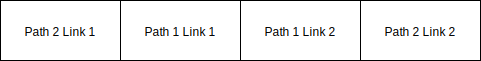
\includegraphics[width=\textwidth]{figures/segmented_links.svg}
    \caption{Path 2 scheduled around Path 1}
    \label{fig:segmented_links}
\end{figure}

The issue with this scenario is that in order to generate path 1, the node requires 2 qubits for generating the two links and having them available at the same time when the SWAP must occur.  When scheduling links for a second path, the algorithm may find that this is a possible ordering.  What need to be taken into consideration is that the node will have at least 3 qubits to perform this.  One for Path 2 Link 1, one for Path 1 Link 1, and one for Path 1 Link 2 since we need to hold Path 2's entanglement through the generation of Path 1's entanglement.

\section{Questions}
\begin{itemize}
    \item What if the slot scheduling algorithm was slot-focused rather than path focused?  Ie, rather than iterating over the set of paths and searching from the available set of slots, iterate over the slots and find an appropriate path from the set to schedule here.
\end{itemize}

\section{Does the order of SWAP matter?}
Three links with fidelities $F_1,F_2,F_3$. Equation for SWAP'd fidelity:

$$F_{new} = F_1F_2 + \frac{(1-F_1)(1-F_2)}{3}$$

Let $F' = F_1 F_2 + \frac{(1-F_1)(1-F_2)}{3}$ be the SWAP'd fidelity of links 1 and 2. Then:

    $$F' F_3 + \frac{(1-F')(1-F_3)}{3}$$
    $$=(F_1 F_2 + \frac{(1-F_1)(1-F_2)}{3})F_3 + \frac{(1-(F_1 F_2 + \frac{(1-F_1)(1-F_2)}{3}))(1-F_3)}{3}$$
    $$=F_1 F_2F_3 + \frac{F_3(1-F_1)(1-F_2)}{3} + \frac{(1-F_1 F_2 - \frac{(1-F_1)(1-F_2)}{3})(1-F_3)}{3}$$
    $$=F_1 F_2F_3 + \frac{(F_3-F_1F_3)(1-F_2)}{3} + \frac{(1-F_3)-F_1 F_2(1-F_3) - \frac{(1-F_3)(1-F_1)(1-F_2)}{3}}{3}$$
    $$=F_1 F_2F_3 + \frac{F_3 - F_2F_3 - F_1F_3 + F_1F_2F_3}{3} + \frac{1-F_3-F_1 F_2+F_1F_2F_3 - \frac{(1-F_3-F_1+F_1F_3)(1-F_2)}{3}}{3}$$
    $$=F_1 F_2F_3 + \frac{1}{3}(1 - F_1F_2 - F_2F_3 - F_1F_3 + 2F_1F_2F_3) - \frac{1}{9}(1 - F_1 - F_2 - F_3 + F_1F_2 + F_2F_3 + F_1F_3 - F_1F_2F_3)$$
    $$=\frac{2}{9} + \frac{1}{9}(F_1 + F_2 + F_3) - \frac{4}{9}(F_1F_2 + F_2F_3 + F_1F_3) + \frac{16}{9}F_1 F_2F_3$$

Substituting fidelities of $1$ in provides what we expect:

$$\frac{2}{9} + \frac{1}{9}(3) - \frac{4}{9}(3) + \frac{16}{9}$$
$$=\frac{2}{9} + \frac{3}{9} - \frac{12}{9} + \frac{16}{9}$$
$$=\frac{5}{9} + \frac{4}{9}$$
$$=1$$

In short, the order of SWAP does \emph{not} matter.  What may matter is if SWAP-ing and holding that link between the two nodes pushes it below a permitted Fidelity due to the rate of decoherence.
\end{document}

\section{TODO}
\begin{itemize}
    \item Check if it is better to generate higher fidelity link first and store it in carbon with slower decoherence or better to store link with lower fidelity in slower decoherence.  Due to the SWAP delay at a node we might want the extra time a higher fidelity link permits us to perform the SWAP rather than using a lower fidelity link that becomes awfully worse during the delay...
    \item Add SWAP noise to link SWAP-ing plots in decoherence.py
    \item Find a way to estimate how much a move to carbon reduces fidelity, or consider supplying initial link fidelity if move occurs from electron to carbon
\end{itemize}